% Exemplo: diagrama de Gantt desenhado em TikZ puro, em uma grade única, com os nomes das
% atividades dentro da moldura e largura igual à do texto.
% Compilar: latexmk -pdf cronograma-gantt.tex     Testado com: abntex2, TikZ, TeX Live 2024 ou mais recente
\documentclass[12pt, a4paper, brazilian]{abntex2}
\usepackage[T1]{fontenc}
\usepackage{tikz}

\begin{document}

A \autoref{fig:gantt} apresenta o cronograma como um diagrama de Gantt.

%%BEGIN:cronogramagantt
\begin{figure}[htbp]
  \caption{Diagrama de Gantt do cronograma do projeto}\label{fig:gantt}
  \centering
  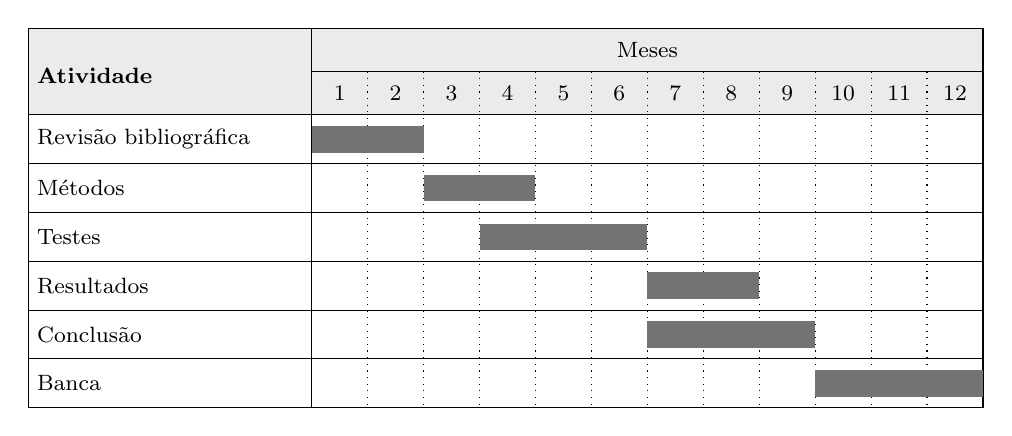
\begin{tikzpicture}[font=\footnotesize, line width=0.4pt]
    \def\gntn{6}                                       % número de atividades
    \pgfmathsetlengthmacro{\gntlc}{3.6cm}              % largura da coluna de atividades
    \pgfmathsetlengthmacro{\gntxu}{(\linewidth-\gntlc)/12} % largura de cada mês
    \pgfmathsetlengthmacro{\gnthh}{1.1cm}              % altura do cabeçalho (2 linhas)
    \pgfmathsetlengthmacro{\gntrh}{0.62cm}             % altura de cada atividade
    \pgfmathsetlengthmacro{\gntht}{\gnthh+\gntn*\gntrh} % altura total
    % cabeçalho sombreado, moldura e linhas
    \fill[black!8] (0,0) rectangle (\linewidth,-\gnthh);
    \draw (0,0) rectangle (\linewidth,-\gntht);
    \draw (0,-\gnthh) -- (\linewidth,-\gnthh);
    \draw (\gntlc,0) -- (\gntlc,-\gntht);
    \draw (\gntlc,-0.55cm) -- (\linewidth,-0.55cm);
    \node[anchor=west, inner xsep=3pt, font=\footnotesize\bfseries] at (0,-0.55*\gnthh) {Atividade};
    \node at ({\gntlc+6*\gntxu},-0.275cm) {Meses};
    \foreach \m in {1,...,12} {
      \node at ({\gntlc+(\m-0.5)*\gntxu},-0.825cm) {\m};
      \draw[dotted] ({\gntlc+\m*\gntxu},-0.55cm) -- ({\gntlc+\m*\gntxu},-\gntht);
    }
    % atividades: nome/mês inicial/mês final
    \foreach \nome/\ini/\fim [count=\k] in {Revisão bibliográfica/1/2, Métodos/3/4,
        Testes/4/6, Resultados/7/8, Conclusão/7/9, Banca/10/12} {
      \pgfmathsetlengthmacro{\yt}{-\gnthh-(\k-1)*\gntrh}
      \draw (0,\yt) -- (\linewidth,\yt);
      \node[anchor=west, inner xsep=3pt] at (0,\yt-0.5*\gntrh) {\nome};
      \fill[black!55] ({\gntlc+(\ini-1)*\gntxu},\yt-0.14cm) rectangle ({\gntlc+\fim*\gntxu},\yt-\gntrh+0.14cm);
    }
  \end{tikzpicture}
  \fonte{Elaborado pelo próprio autor.}
  \nota{Cada barra indica a duração da atividade, em meses.}
\end{figure}
%%END:cronogramagantt

\end{document}
